%iso-8859-2 encoding
\chapwithtoc{Opengl-Android application, Knots animator} % (fold)
\label{cha:Opengl-Android application}
\url{http://code.google.com/p/opengl-android/}

\section*{Problem definition} % (fold)
\label{sec:Problem definition}
Climbers have to use knots a lot. It is difficult to learn them all
and it is even harder to explain it by words.

I experienced few times a situation when pair of climbers
were arguing how to bind a knot before belaying each other
30 meters above a ground.

It will be really handy to have not only a learning tool
how to bind all necessary knots, but also a reference, 
which can be understandable quickly to every one.
% section* Problem definition (end)

\section*{User stories} % (fold)
\label{sec:User stories}
\begin{itemize}
  \item As a user, I want to press a button and launch Knot animator. 
  \item As a user, I want in running Knot animator press options button and view settings.
  \item As a user, I want to choose knots via "Knot selections" in opened settings.
  \item As a user, I want to set up Knot animator as a screen saver by pressing button in opened settings.
  \item As a user, I want to press the cancel button in order to see the last knot.
  \item As a user, I want to view knot in 3D after choosing the knot.
  \item {\bf Starting application:} After start, a user will see a default knot in 3D as if he chose it manually.
  \item As a user, I want to set up the default knot on the screen launched from the opened settings.
  \item {\bf Launching animation:}  As a user, I want to just click the display knot in order to see the animation how the knot is binded.
  \item {\bf Pausing animation:} As a user, I want to click the display to stop the animation.
  \item {\bf Canceling the animation:} As a user, I want to press the cancel button in order to stop the animation and back display the knot.
  \item {\bf Exiting the application:} As a user, I have to see one of the knots and press cancel button. 
\end{itemize}

% section User stories (end)

\section*{Solution and description of the project} % (fold)
\label{sec:Solution}
The aim of this application is to be an always ready advisor, which will
present even to a child how a knot can be bind. 

"Knots animator" should  allow users to display the set of knots from different angle
and furthermore the application should offer rendering of knots binding.

Different points of view together with colourisation of the knots bindings
allows user to more easily understand how one the knots are binded.
In order to achieve good quality of 3D rendering, "Knots animator" 
uses OpenGL ES and also a full screen mode. 
The option of running the application as a screen saver could be really interesting
for passionate climbers.

Last but not least the application loads knots definitions from a XML files,
which allows application easily deploy additional sets of knots to customers.
Moreover the users can define knot on their own.
% section* Solution (end)

\section*{Target users} % (fold)
\label{sec:Target users}
Target users can be found among climbers and outdoor lovers,
which likes nicely looking and simple to use applications.  
I suppose that especially climbing instructors will appreciate
to have additional learning tool.
% section* Target users (end)

\section*{Technology used} % (fold)
\label{sec:Technology used}

\begin{itemize}
  \item Android - target platform 
  \item Android SDK - Java framework for Android
  \item Android NDK - Native framework for Android
  \item OpenGL ES 1.0 - graphical engine restricted to Android
  \item XML - definition language 
\end{itemize}

The Knot animator is an Android application, 
thats user interface was developed by using Android SDK framework.
Nevertheless the crucial part of knot rendering uses OpenGL ES 1.0,
which is a little restricted OpenGL graphical engine for Android devices.

As we decided to render 3D graphics, the choice of OpenGL came naturally.
The OpenGL ES 1.0 engine provides both necessary functionality and due to
native implementation also a better performance.

In order to interface OpenGL we use JNI (Java Native Interface) wrapper.
You can learn more about why we do not access directly fro Java in Subsection ~\ref{Used technology}.

% section* Technology used (end)

\section*{Architecture} % (fold)
\label{sec:Architecture}
The Knot animator has simple application logic with clearly divided tasks.
\begin{itemize}
  \item First of all we store the knot definitions in XML files,
so the Knot animator has to able parse the definition XML file of every knot.
  \item Secondly in order to interact with user input and other applications the application 
  implements Activities \todo{ TodoActivity1}, \todo{TodoActivity2}.
  \item The crucial part of application is rendering the 3D animation. We use OpenGL ES 1.0,
      JNI in classes \todo{TODO viewerGL} \todo{JNI wrapper}.
\end{itemize}

\todon{ graph of classes}
\todon{application logic graph}


\section*{Features and Effort} % (fold)
\label{sec:Features and Effort}
Obviously the key feature is to render the knot in 3D using OpenGL ES.
However, OpenGL ES could be used in two different ways on Android platform.

The first possibility is to call OpenGL functions through Java wrapper.
Java wrapper allows programmers to avoid C/C++ programming of OpenGL.
On the other hand, problems with passing parameters, especially preallocated arrays,
force to use programmers to use workarounds.

The second attitude is to use JNI. JNI is also a Java wrapper around C/C++ but does not wrap the OpenGL,
but the whole application logic in class {\it Activity}. 
The possibility to handle application in C/C++ allows developers call OpenGL ES directly from C/C++.

We have chosen to use the second attitude and implement 3D rendering using OpenGL ES and JNI.
The main reasons are:
\begin{itemize}
  \item Clear interface between OpenGL ES and Android application
  \item Possible performance improvement
  \item Possibility of code reuse (I would like to build classic OpenGL app in C)
  \item Learning JNI
\end{itemize}

However the crucial part of this application lies 
in choosing the right data representation for storing the shape of knots.

I expect most problems in designing as well as parsing XML file
for storage of the 3D visualisation.

Others features like full screen invocation or animation selection
I consider not application specific and I expect
to use classical techniques of Android programming.

The "nice to have" features like animation colourising 
or viewpoint change are not crucial for making decision
about architecture of this application. 
I also expect, that their implementation will consume minor time
in meaning of the whole project.

\begin{tabular}{| l || c | c |  c | c |}
\hline
Feature & Priority & Implemented & Est. hours & Real hours\\
\hline
\textbf{Learning JNI} & high & NO & 4 & 1\\
\textbf{Exploring ndk samples} & high & NO & 12 & 4\\
\textbf{Design of XML} & high & NO & 15 & 1.5\\
\textbf{OpenGL demo} & high & NO & 4 & ?\\
\textbf{Running animation} & high & NO & 20 & ?\\
\textbf{Loading XML definition} & high & NO & 6 & ?\\
\textbf{Select animation} & high & NO & 1 & ?\\
\textbf{Full screen} & middle & NO & 3 & ?\\
\textbf{Screen saver} & middle & NO & 4 & ?\\
\textbf{Binding colourising} & middle & NO & 4 & ?\\
\textbf{Viewpoint manual} change & low & NO & 2 & ?\\
\textbf{Docs \& refactoring} & middle & NO & 5 & 0\\
\hline
\end{tabular}
\begin{figure}
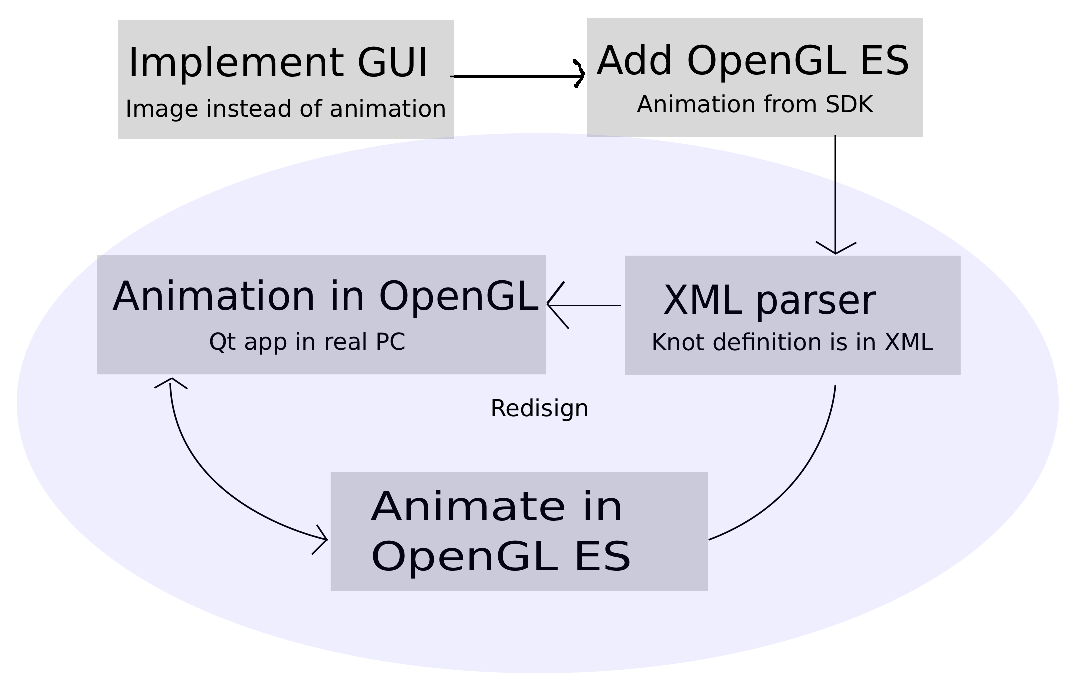
\includegraphics{work_flow.eps}
\label{work_flow}
\caption{Work flow}
\end{figure}

\todon{workflow of activities with dependecies}
\todon{ait/project/samples/san-angeles      DemoActivity    OpenGL 1.0}
\todon{ait/project/samples/hello-gl2        GL2JNIActivity  OpenGL 2.0   does not run on emulator}
% section* Features and Effort (end)

\section*{Technical problems} % (fold)
\label{sec:Technical problems}
\todon{write summary technical problems}
% section* Technical problems (end)

\subsection*{Used technology and design problems} % (fold)
\label{sub:Used technology}
 At the beginning of this project, the decision abou
 \todon{describe decisions about choosing OpenGL 1 vs 2. Xml parsing and knot animating}
% subsection Used technology (end)

\subsection{Tools and Hardware problems} % (fold)
\label{sub:Hardware problems}
\todon{write about android adt, not supported simulator 2.0 etc} 
% subsection Hardware problems (end)


\section*{Additional freatures} % (fold)
\label{sec:Additional freatures}
 Really nice feature could be tightening the knot during its binding.
 Another possibility how to enrich this application is to implement
 a voice advisor, who will give you spoken instruction during the animation.

% section* Additional freatures (end)
% chapter Opengl-Android application (end)
